\documentclass[a4paper]{article}
\let\proof\relax
\let\endproof\relax
\usepackage[utf8]{inputenc}
\usepackage[T1]{fontenc}
\usepackage{textcomp}
\usepackage{mathtools,amssymb,amsthm}
\usepackage{lmodern}
\usepackage{geometry}
\geometry{hmargin=3cm,vmargin=3cm}
\usepackage{amsmath,amsfonts,amssymb}
\usepackage{tikz}
\usepackage{fancyhdr}
\usepackage{eso-pic}
\usepackage{xcolor}
\usepackage{listings}
\usepackage{booktabs}
\usepackage{setspace}
\usepackage{caption}
\usepackage{subcaption}
\usepackage{graphicx}
\definecolor{mGreen}{rgb}{0,0.6,0}
\definecolor{mGray}{rgb}{0.5,0.5,0.5}
\definecolor{mPurple}{rgb}{0.58,0,0.82}
\definecolor{backgroundColour}{rgb}{0.95,0.95,0.92}

\lstdefinestyle{customc}{
  belowcaptionskip=1\baselineskip,
  breaklines=true,
  frame=L,
  xleftmargin=\parindent,
  language=C,
  showstringspaces=false,
  basicstyle=\footnotesize\ttfamily,
  keywordstyle=\bfseries\color{green!40!black},
  commentstyle=\itshape\color{purple!40!black},
  identifierstyle=\color{blue},
  stringstyle=\color{orange},
}

\lstset{escapechar=@,style=customc}
\onehalfspacing

\begin{document}




\AddToShipoutPicture{%
  \AtPageLowerLeft{%
    \rotatebox{90}{\colorbox{gray!20}{%
      \begin{minipage}{\paperheight}\sffamily 
      \hspace*{\stretch{1}} \textbf{Rapport Projet S5: MANSUBA.}\hspace*{\stretch{1}}
      \end{minipage}%
    }}%
  }%
}


\title{  
\includegraphics[scale=0.09]{logo.png} \\ \underline{Rapport de projet S5:} \\ \textbf{MANSUBA} \\$\newline$ 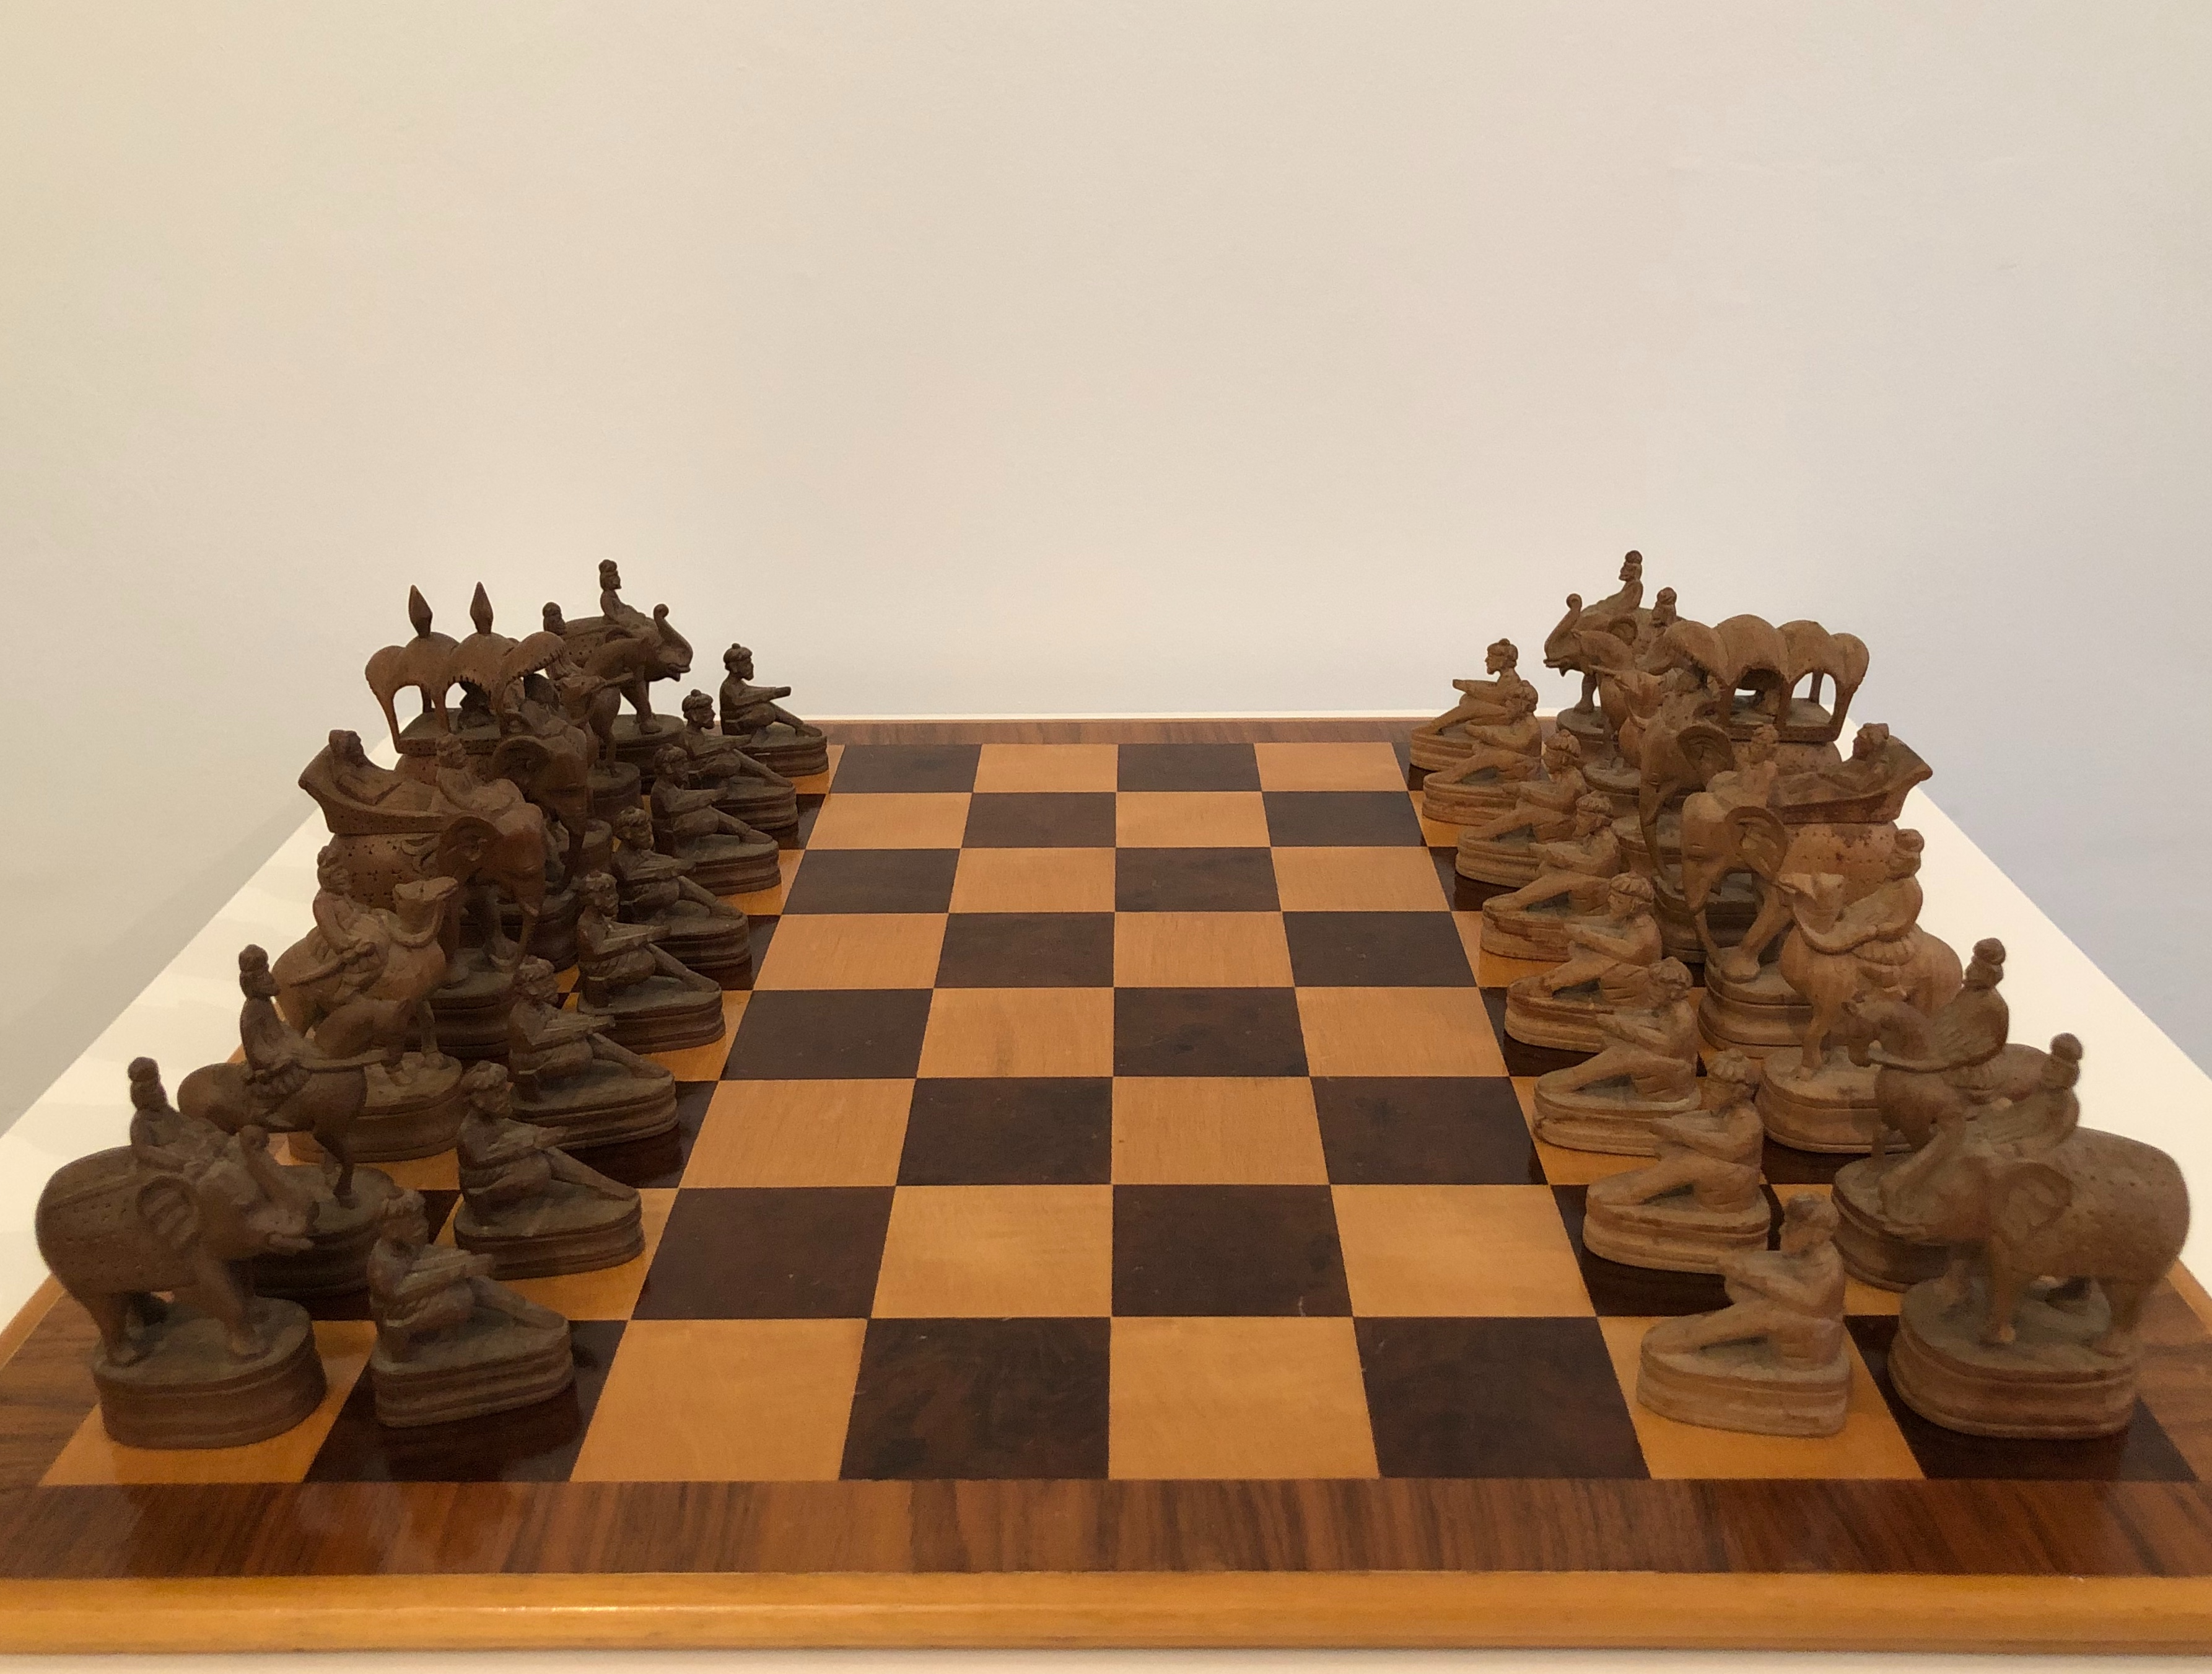
\includegraphics[scale=0.1]{Chaturanga_Chess_Set.jpg} }


\author{Réalisé par:\\MOHAMMED BOUHAJA ET AMIRA ELOUAZZANI \\\textbf{Encadré par: Julien Allali}}
\date{}
\maketitle





\newpage



\tableofcontents 


\newpage




  


\section{Introduction}
\subsection{Problèmatique}
$\newline$
$\hspace*{0.7cm}$Mansuba est un jeu de plateau , ancêtre de Shtranj , qui a comme but mettre l’autre joueur en situation de mat . 
Le but de notre projet sera de jouer une partie aléatoire avec plusieurs configurations.

La programmation d'un tel jeu est un défi qui nécessite une compréhension approfondie des règles et des
stratégies du jeu, ainsi qu'une maîtrise des concepts de programmation tels que la gestion de la mémoire,
la récursivité et les algorithmes de recherche. L'un des principaux défis est de concevoir un système d'évaluation des positions pour évaluer
 la performance des différentes stratégies. Cela peut être difficile car il faut déterminer les facteurs importants
  à considérer et comment les pondérer. Il est également important dans la programmation de ce projet est de concevoir
   un système de mouvement de pièces efficace et logique. Il est nécessaire de définir des règles pour les mouvements valides de
    chaque type de pièce, ainsi que de prendre en compte les situations de pat et de mat.


\subsection{Manusba}

$\hspace*{0.7cm}$Pour jouer une partie, il faut que le plateau de jeu soit défini au préalable. Le plateau de jeu \textit{board}  est 
le binôme monde et relation. 
Le monde \textit{world} est l’ensemble des cases accessibles par les pions . Chaque case a 
désormais des cases voisines \textit{Neighbors} dans différentes directions.
La possibilité d’accès à ses voisins sera contrôlée par la relation de la partie qui choisira parmis les voisins ceux qui sont
 accessibles .  
Les pièces selon leurs types (pions, éléphant, tour) admettent différents types de mouvements : déplacement simple, saut simple, saut diagonal ... .
Il existe deux types de victoires. La victoire est dite simple si le joueur atteint une des positions de départ de l’autre joueur
 et complexe si le joueur les atteint tous.
Le jeu s’arrête si on atteint une victoire, le choix du type étant aléatoire pendant la partie, ou si on atteint le nombre de tour maximal. 


\subsection{Travail en binôme, git}

Travailler en binôme sur un projet de programmation peut offrir de nombreux avantages tels que la répartition
 des tâches et la révision de code, mais il est important d'utiliser des outils pour faciliter la gestion des versions
  et la communication, L'un de ces outils est le Git qui permet de suivre les modifications apportées au code et gérer les conflits potentiels.

\section{Implémentation}

$\hspace*{0.7cm}$Le jeu s’effectue dans un monde de $\textcolor{purple}{\textsc{world\_size}} = \textcolor{purple}{\textsc{width}} \times 
 \textcolor{purple}{\textsc{height}}$  cases , avec des pièces appartenant à un nombre de joueurs \textcolor{purple}{\textsc{max\_players}}.
. Cette configuration est surtout gouvernée par \textcolor{green}{\textit{geometry.h}} qui donne \lstinline|enum color_t| et \lstinline|enum sort_t|. \\


On s'intéresse dans notre projet à plusieurs structure de base dans la construction de projet , parmi eux des structures statiques qui
nécessite un accés indirecte.

Pendant le développement du jeu on fera souvent appel à toute la configuration du jeu. On rassemble alors tous les paramètres du monde
 pendant le jeu dans une structure \lstinline|struct game_t|.
\begin{lstlisting}
struct game_t {
    enum color_t current_player;
    unsigned int tour;
    struct world_t* w;
    struct jail_t* jail;
    unsigned int seed;
    unsigned int position;
    enum victory_t victory;
};
\end{lstlisting}


Pour jouer une partie aléatoire on aura besoin de configurer le plateau de jeu.


\subsection{Partie monde}

$\hspace*{0.7cm}$La structure world est un tableau de pair couleur et type de pions qui inaccessible que par des fonctions de 
\textcolor{green}{\textit{world.h}}. On commence d’abord par initier un monde sans aucun pion à l’aide de la fonction
\lstinline|struct world_t* world_init()|. Les fonctions de world.h permettront l’écriture et la lecture de la couleur et
 du type d’une case donné et seront utilisé fréquemment pour accéder au monde.  
 
 \begin{center}
 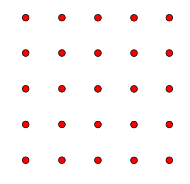
\includegraphics[scale=0.4]{5.png}{\\$\hspace*{0.7cm}$Figure x: Un monde}
 \end{center}

\subsection{Partie relation}

La structure \lstinline|struct neighbors_t| prédéfinira les voisins de chaque indice donné . 
\begin{lstlisting}
struct neighbors_t {
  struct vector_t n[MAX_NEIGHBORS+1];
};
\end{lstlisting}

\begin{center}
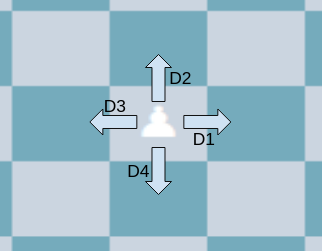
\includegraphics[scale=0.5]{movespawn2.png} {\\$\hspace*{0.7cm}$Figure x: }
\end{center}


Les voisins seront un tableau précalculé dont le contenu pour un indice donné de taille \textcolor{purple}{\textsc{max\_neighbors}} . De la même façon que world, les fonctions qui donne 
 accès au voisins sont \lstinline|struct neighbors_t get_neighbors(unsigned int idx)| qui cherche dans la structure des voisins 
 l’élement d’indice rentré en paramètre et \lstinline|unsigned int get_neighbor(unsigned int idx, enum dir_t d)|qui aide à obtenir 
 le voisin dans une direction donné par des opérations sur l’indice.\\ 

L’initialisation d’une relation modifie la liste des voisins pour qu’il puisse inclure que des voisins de certain directions donné. 
Avant d’initialiser une relation on pose dans la structure neighbors comme premier voisin pour chaque indice le pair 
\textcolor{purple}{\textsc{(uint\_max , no\_dir)}} et un (0,0) pour le reste. \textcolor{purple}{\textsc{uint\_max}} est définie 
dans \textcolor{green}{\textit{limits.h}}. La fonction add\_neighbor servira par suite à pousser \textcolor{purple}{\textsc{(uint\_max , no\_dir)}} 
et le remplacer par le pair indice du voisin et sa direction.
Le paramètre \textit{seed} permettera de désigner la relation de la partie et sera modifiable à $\sqrt{\textsc{max\_turns}}$. On donne le choix entre 4 relations : simple, diagonale, triangulaire, hexagonal.

\begin{figure}
  \centering
  \begin{minipage}{.5\textwidth}
    \centering
    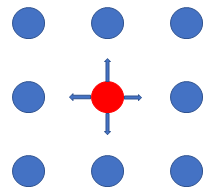
\includegraphics[width=.4\linewidth]{1.png}
    \captionof{figure}{relation simple}
    \label{fig:test1}
  \end{minipage}%
  \begin{minipage}{.5\textwidth}
    \centering
    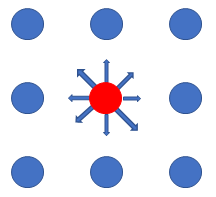
\includegraphics[width=.4\linewidth]{2.png}
    \captionof{figure}{relation diagonale}
    \label{fig:test2}
  \end{minipage}
  \end{figure}


  \begin{figure}
    \centering
    \begin{minipage}{.5\textwidth}
      \centering
      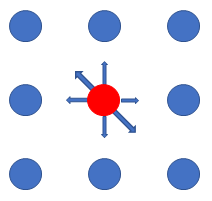
\includegraphics[width=.4\linewidth]{3.png}
      \captionof{figure}{relation triangulaire}
      \label{fig:test1}
    \end{minipage}%
    \begin{minipage}{.5\textwidth}
      \centering
      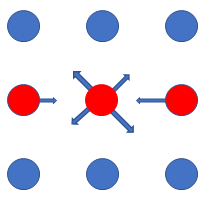
\includegraphics[width=.4\linewidth]{4.png}
      \captionof{figure}{relation hexagonale}
      \label{fig:test2}
    \end{minipage}
    \end{figure}

\subsection{Ensemble}
\begin{lstlisting}
\subsection{Ensemble}
\begin{lstlisting}

struct set{
    unsigned int taille;
    unsigned int positions[WORLD_SIZE];
};
\end{lstlisting}
Cette structure \lstinline|struct set|  permettra de construire des tableaux d’une taille donnée et simplifier leurs 
manipulations : lecture et écriture , comme le jeu a plusieurs collections à fournir : l’set des positions des pions, la 
collection des mouvement possibles  ... . 


\subsection{mouvements des pièces}


\subsubsection{Mobilité d'un pion \textit{PAWN}}
Pour stocker les mouvements on fera appel à la structure set . Les mouvement possibles dans la version de bases sont :  

    \textbf{\textcolor{magenta}{Déplacement simple}} : Déplacement vers une case directement voisine libre.
    
\begin{center}
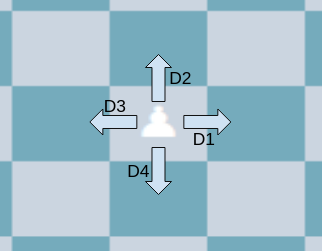
\includegraphics[scale=0.5]{movespawn2.png} {\\$\hspace*{0.7cm}$Figure x: Déplacement simple d'un pion.}
\end{center}

$\newline$

    \textbf{\textcolor{magenta}{Saut simple}} : si le voisin dans une direction j est occupé, et le voisin du voisin dans la meme direction est libre ,  on peut se déplacer vers le voisin du voisin , si le monde le permet. 

    \begin{center}
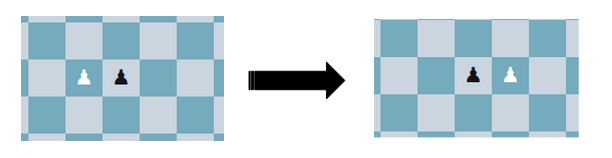
\includegraphics[scale=0.6]{sautf.png} {\\$\hspace*{0.7cm}$Figure x: Saut simple d'un pion.}
\end{center}

$\newline$

    \textbf{\textcolor{magenta}{Saut multiple}} : s’agit d’une suite de saut simple dans different direction. elle est implémenté récursivement. La condition d’arrêt pour éviter de boucler infiniment sur les sauts simples est que les deux voisins soient occupés , arrête la boucle dans une direction , ou que l'indice soit déjà visité par notre fonction . 
    
\begin{center}
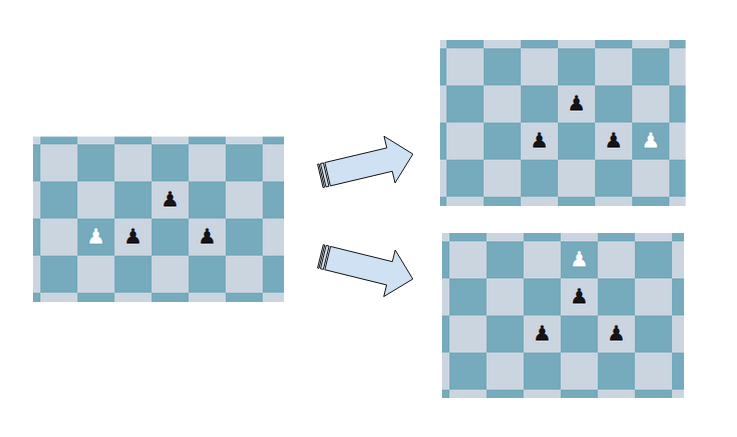
\includegraphics[scale=0.6]{sautmf.png} {\\$\hspace*{0.7cm}$Figure x: Saut multiple d'un pion.}
\end{center}

La fonction multiple$\_$jumps utilise une récursion qui augmente sa complexité de manière exponentielle, cependant elle
utilise aussi une fonction simple$\_$jumps qui elle est de complexité constante. Ce qui donne une complexité globale de
la fonction multiple$\_$jumps qui est exponentielle avec une constante dépendant de la fonction simple$\_$jumps sachant que
 les autres fonctions utilisées sont de complèxité constante.

$\newline$

Ses fonctions prennent comme paramètre additionnel un set. Il servira comme espace de stockage . 

\subsubsection{Mobilité des autre pièces \textit{TOWER} et \textit{ELEPHANT }}

$\newline$

\textbf{\textcolor{magenta}{Translation cardinale}} : La tour se déplace en ligne droite soit horizontalement soit verticalement 
de tout nombre de cases inoccupées, donc on réalise une boucle sur les quatres direction SOUTH, NORTH, EAST et WEST, jusqu'à ce
 qu'elle atteigne le bord de l'échiquier ou qu'elle soit bloquée par une autre pièce. Elle ne peut passer au dessus d'une
  autre pièce.

\begin{center}
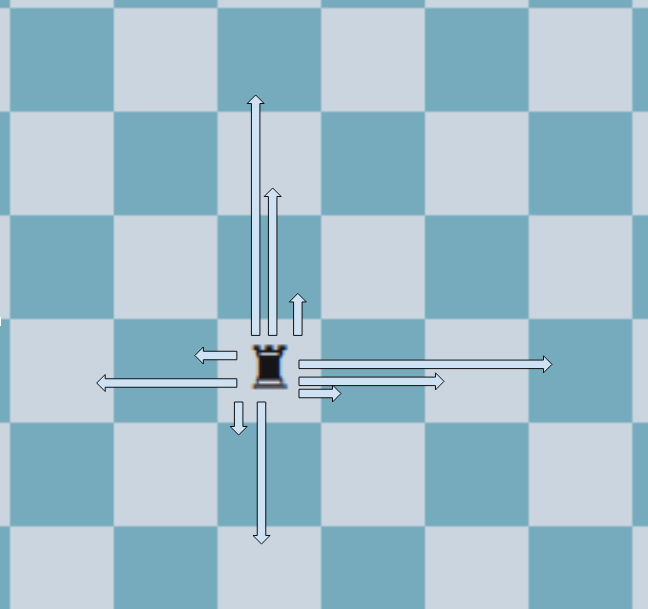
\includegraphics[scale=0.3]{tour2.png} {\\$\hspace*{0.5cm}$Figure x: Translation cardinal d'une tour.}
\end{center}

$\newline$

\textbf{\textcolor{magenta}{Saut semi diagonal}} : L'éléphant peut se déplacer sur les deux diagonale à partir de sa position initial, pour ce faire on boucle sur les directions $i+j$ $(où ~i \in \{NORTH, ~SOUTH\} ~et~ j \in \{ EAST, ~WEST \})$ et on ajoute les positions libres. finalement on stocke le résultat dans un ensemble $sdj$.

\begin{center}
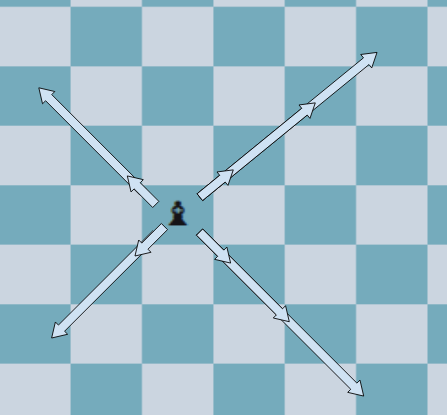
\includegraphics[scale=0.45]{ele2.png} {\\$\hspace*{0.4cm}$Figure x: Saut semi diagonal de l'éléphant.}
\end{center}


\subsubsection{Possibilité de capture et les tentatives d'évasion}
$\newline$
Les mobilités des pièces ont un rôle très important dans notre jeu, mais ceci rend le jeu un peu statique où le nombre de pièces reste le même du début jusqu'à la fin. Donc on va améliorer ça en ajoutant d'une part des captures simples qui permettent par exemple dans un jeu d'echecs de retirer les pièces les plus fortes de l'adversaire, affaiblissant ainsi sa position et peut également permettre de créer des opportunités et des ouvertures pour les pièces restantes, d'autre part la possibilité de s'évader pour une pièces prisonnière. 

$\newline$

\textbf{\textcolor{magenta}{Capture simple}} : Une capture simple pour être définie comme tout déplacement d'une pièce qui aboutit sur une case occupée par une pièce d'une couleur opposée entraîne la capture de cette dernière (prisonnère), et on stocke ces captures dans des ensembles pour chaque type de pièce donné.


$\newline$

Une pièce capturée deveint prisonnière, pour gerer cette nouvelle implémentation on crée une structure \textit{prisoner\_t} qui décrit l'état de la pièce capturée et pour manipuler plusieurs prisonèrs on définie une structure \textit{jail\_t} qui contient les différents prisonèrs des deux joueurs. les deux structures sont définie de la manière suivante:


\begin{lstlisting}

struct prisoner_t{
  enum color_t c;
  enum sort_t s;
  unsigned int i;
};

struct jail_t{
  unsigned int len_white;
  unsigned int len_black;
  struct prisoner_t cells_white[WORLD_SIZE];
  struct prisoner_t cells_black[WORLD_SIZE];
};
\end{lstlisting}




Mais pour ajouter une nouvelle dimension au jeu on implémente la posibilité d'évasion.

\textbf{\textcolor{magenta}{Tentatives d'évasion}} : Si une pièce est capturée, elle a la possibilité de tenter de s'échapper. Cependant, cette évasion n'est possible que si la case où elle a été capturée est vide. La réussite de cette évasion est aléatoire, avec une chance de 50$\%$ de réussir. Si l'évasion échoue, la pièce reste capturée et le plateau de jeu reste inchangé.


\begin{center}
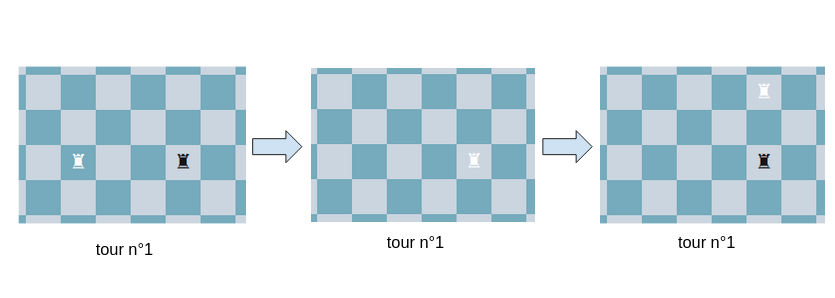
\includegraphics[scale=0.5]{evasion.png}{\\$\hspace*{1.5cm}$Figure: Évasion d'une pièce.}
\end{center}
$\newline$

\subsection{Graphe des inclusions}

$\newline$

\begin{center}
  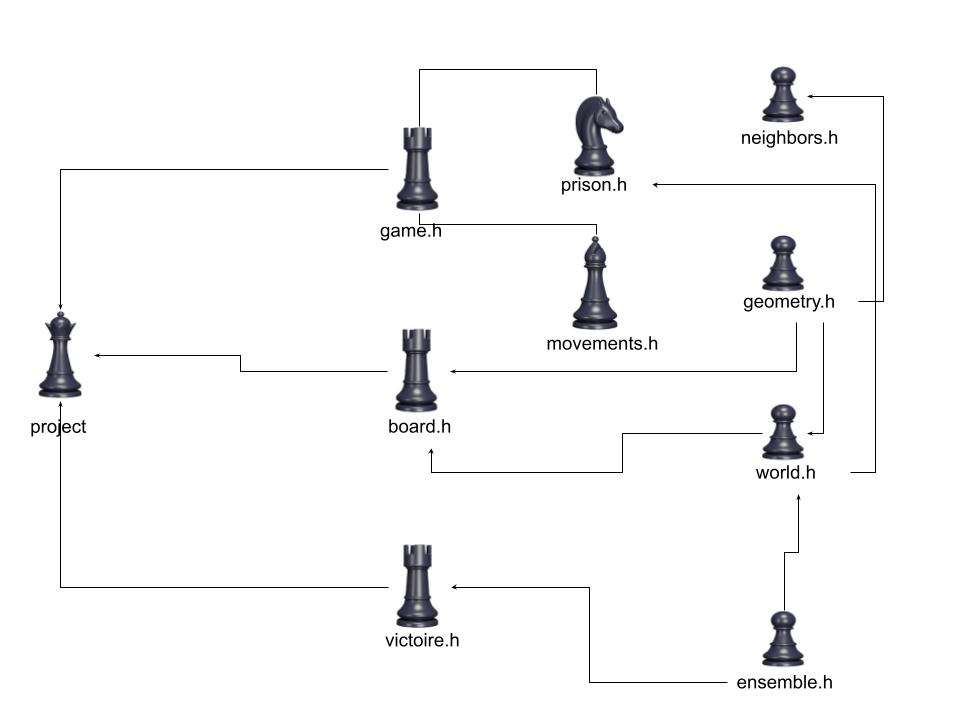
\includegraphics[scale=0.5]{Dessin sans titre.jpg}
\end{center}

\section{Configuration de compilation et exécution}
\subsection{Makefile}


Les fichiers .c  ont été construit et exécuté à l'aide d'un Makefile. Ce fichier de configuration automatise les tâches de compilation et d'exécution, facilitant ainsi la maintenance et l'extensibilité du logiciel. Les options de compilation et les dépendances ont été définies dans le Makefile, ainsi que les cibles pour construire et exécuter le programme. Nous avons utilisé GNU Make, un outil populaire pour créer des Makefiles, pour créer le Makefile de ce projet. En cours de développement, nous avons rencontré des problèmes avec les dépendances de bibliothèques, qui ont été résolus en ajoutant des options de compilation supplémentaires dans le Makefile. La méthodologie de compilation et d'exécution décrite ici a permis un développement efficace et une exécution stable de tous les fichiers.

\subsection{La manipulation des options de ligne de commande}


Pour manipuler la ligne de commande on a utiliser $getopt$, c'est un moyen efficace pour la gestion des optiosn et des arguments lors de la compilation du projet, donc l'utilisation de getopt nous a permis de rendre le terminal une interface utilisateur intuisive et personnalisable. Il utilise une bibliothèque standard $getopt$ de C. Se qui nous a permis de définir avant l'éxusion du projet le type de victoire souhaité par l'utilisateur, le nombre de tours et le nombre qui génére $rand()$. 

La bibliothèque getopt en C utilise la fonction getopt() pour analyser les options et les arguments passés à un programme lors de son exécution. Cette fonction prend en entrée les arguments standard argc et argv du programme, ainsi qu'une chaîne de caractères optstring qui définit les options valides pour le programme.

La fonction getopt() analyse ensuite les arguments dans argv en utilisant les options définies dans optstring. Pour chaque option valide détectée, getopt() retourne le caractère correspondant. Si une option nécessite un argument, celui-ci est stocké dans la variable globale optarg.

Les options peuvent être spécifiées de différentes manières. Les options courtes sont des caractères simples précédés d'un tiret (par exemple: -t pour le type de victoire et -m pour le nombre de tours). Les options longues sont des chaînes de caractères précédées de deux tirets (par exemple: --option).

Après avoir analysé tous les arguments, getopt() retourne -1 pour indiquer qu'il n'y a plus d'options valides. Les développeurs peuvent utiliser cette valeur pour itérer sur les options et les arguments restants.

Il est important de noter que getopt() modifie l'ordre des éléments dans argv pour les options traitées. Les arguments restants sont décalés vers le début de la liste argv.


\section{Conclusion}


\end{document}